% Style Transfer — Hierarquia de Características na CNN (Grelha Corrigida)
% Uso: % Style Transfer — Hierarquia de Características na CNN (Grelha Corrigida)
% Uso: % Style Transfer — Hierarquia de Características na CNN (Grelha Corrigida)
% Uso: % Style Transfer — Hierarquia de Características na CNN (Grelha Corrigida)
% Uso: \input{resources/style-transfer/cnn-hierarchy.tex}
\begin{figure}[htbp]
\centering
\resizebox{\textwidth}{!}{%
\begin{tikzpicture}[
    >=latex,
    layer/.style={draw=wp-text, rounded corners=2pt, minimum width=3.0cm, minimum height=1.2cm, align=center, font=\small},
    conn/.style={->, draw=wp-primary, thick},
    brk/.style={decorate, decoration={brace, amplitude=5pt}, draw=wp-muted, thick},
    tuftebox/.style={draw=wp-light, fill=wp-code, rounded corners=2pt, align=center}
]

% =========================================================================
% FLUXO PRINCIPAL: CAMADAS DA CNN (Eixo X Otimizado)
% =========================================================================

\node[layer, fill=wp-accent!15, draw=wp-accent] (conv1) at (3.5, 2.5) {Camadas Iniciais\\conv$_1$ -- conv$_2$};
\node[layer, fill=wp-primary!10, draw=wp-primary] (conv2) at (7.0, 2.5) {Camadas Médias\\conv$_3$ -- conv$_4$};
\node[layer, fill=wp-text!10, draw=wp-text] (conv3) at (10.5, 2.5) {Camadas Profundas\\conv$_5$ -- conv$_6$};

% Imagem de Entrada simplificada para apenas "X"
\node[draw=wp-text, fill=wp-code, rounded corners=2pt, minimum width=1.0cm, minimum height=1.0cm, align=center, font=\large\bfseries] (input) at (0.8, 2.5) {$\mathcal{I}$};

% Conexões do Fluxo Principal
\draw[->, draw=wp-primary, thick] (input.east) -- (conv1.west);
\draw[->, draw=wp-primary, thick] (conv1.east) -- (conv2.west);
\draw[->, draw=wp-primary, thick] (conv2.east) -- (conv3.west);


% =========================================================================
% VISUALIZAÇÕES DE RECURSOS (Aproximadas verticalmente)
% =========================================================================

\node (vis1) at (3.5, 1.1) {
  \begin{tikzpicture}[scale=0.3]
    \foreach \i in {0,...,4}
      \foreach \j in {0,...,4}
        \pgfmathparse{mod(\i+\j,2)*100}
        \fill[black!\pgfmathresult] (\i*0.5, -\j*0.5) rectangle ++(0.45, 0.45);
  \end{tikzpicture}\quad
  
\begin{tikzpicture}[scale=0.3]
    \foreach \i in {0,...,4}
      \foreach \j in {0,...,4}
        \pgfmathparse{int(rnd*100)}
        \fill[black!\pgfmathresult] (\i*0.5, -\j*0.5) rectangle ++(0.45, 0.45);
  \end{tikzpicture}\quad
  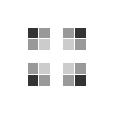
\begin{tikzpicture}[scale=0.3]
    \foreach \i in {0,...,4}
      \foreach \j in {0,...,4}
        \pgfmathparse{abs(\i-2)*abs(\j-2)*20}
        \fill[black!\pgfmathresult] (\i*0.5, -\j*0.5) rectangle ++(0.45, 0.45);
  \end{tikzpicture}
};

\node (vis2) at (7.0, 1.1) {
  
\begin{tikzpicture}[scale=0.3]
    \foreach \i in {0,...,4}
      \foreach \j in {0,...,4}
        \pgfmathparse{sin(deg(\i*1.5+\j*1.5))*50+50}
        \fill[black!\pgfmathresult] (\i*0.5, -\j*0.5) rectangle ++(0.45, 0.45);
  \end{tikzpicture}\quad
  
\begin{tikzpicture}[scale=0.3]
    \foreach \i in {0,...,4}
      \foreach \j in {0,...,4}
        \pgfmathparse{cos(deg(\i*2))*cos(deg(\j*2))*50+50}
        \fill[black!\pgfmathresult] (\i*0.5, -\j*0.5) rectangle ++(0.45, 0.45);
  \end{tikzpicture}\quad
  
\begin{tikzpicture}[scale=0.3]
    \foreach \i in {0,...,4}
      \foreach \j in {0,...,4}
        \pgfmathparse{sin(deg(sqrt(\i^2+\j^2)*2))*50+50}
        \fill[black!\pgfmathresult] (\i*0.5, -\j*0.5) rectangle ++(0.45, 0.45);
  \end{tikzpicture}
};

\node (vis3) at (10.5, 1.1) {
  
\begin{tikzpicture}[scale=0.3]
    \foreach \i in {0,...,4}
      \foreach \j in {0,...,4}
        \pgfmathparse{\i==2 && \j==2 ? 80 : 10}
        \fill[black!\pgfmathresult] (\i*0.5, -\j*0.5) rectangle ++(0.45, 0.45);
  \end{tikzpicture}\quad
  
\begin{tikzpicture}[scale=0.3]
    \foreach \i in {0,...,4}
      \foreach \j in {0,...,4}
        \pgfmathparse{(\i-2)^2+(\j-2)^2 < 2 ? 80 : 10}
        \fill[black!\pgfmathresult] (\i*0.5, -\j*0.5) rectangle ++(0.45, 0.45);
  \end{tikzpicture}\quad
  
\begin{tikzpicture}[scale=0.3]
    \foreach \i in {0,...,4}
      \foreach \j in {0,...,4}
        \pgfmathparse{(\i==1 || \i==3) && (\j>=1 && \j<=3) ? 80 : 10}
        \fill[black!\pgfmathresult] (\i*0.5, -\j*0.5) rectangle ++(0.45, 0.45);
  \end{tikzpicture}
};

% --- SETAS PONTILHADAS ---
\draw[->, draw=wp-muted, thick, dashed] (conv1.south) -- (vis1.north);
\draw[->, draw=wp-muted, thick, dashed] (conv2.south) -- (vis2.north);
\draw[->, draw=wp-muted, thick, dashed] (conv3.south) -- (vis3.north);


% --- TEXTOS INFERIORES DE CARACTERÍSTICAS ---
\node[font=\footnotesize, align=center, text=wp-accent] at (3.5, -0.1) {Bordas\\Texturas\\Cores};
\node[font=\footnotesize, align=center, text=wp-primary] at (7.0, -0.1) {Padrões\\Partes\\Formas simples};
\node[font=\footnotesize, align=center, text=wp-text] at (10.5, -0.1) {Objetos\\Semântica\\Conceitos};


% --- CHAVES SUPERIORES (Braces) ---
\draw[brk] (5.1, 4.0) -- (1.9, 4.0);
\node[above=4pt, font=\small, text=wp-accent] at (3.5, 4.0) {ESTILO (baixo nível)};

\draw[brk] (8.6, 4.0) -- (5.4, 4.0);
\node[above=4pt, font=\small, text=wp-primary] at (7.0, 4.0) {transição};

\draw[brk] (12.1, 4.0) -- (8.9, 4.0);
\node[above=4pt, font=\small, text=wp-text] at (10.5, 4.0) {CONTEÚDO (alto nível)};


% =========================================================================
% BLOCO SUPERIOR RE-ALINHADO E PROPORCIONAL
% Centrado exatamente em x=7.0 (meio do gráfico) com largura equilibrada de 7.0cm
% =========================================================================
\node[tuftebox, minimum width=7.0cm, minimum height=1.2cm] at (7.0, 6.0) {
    \textbf{\color{wp-primary}\small Extração de Características e Perdas}\\[4pt]
    \footnotesize Perda de estilo: múltiplas camadas (baixo + médio)\\
    \footnotesize Perda de conteúdo: camada profunda (alto nível)
};

\end{tikzpicture}
}
\caption{Hierarquia de características em uma CNN. Camadas iniciais capturam bordas, texturas e cores (estilo). Camadas médias detectam padrões e partes de objetos. Camadas profundas representam objetos completos e semântica de alto nível (conteúdo). A perda de estilo utiliza múltiplas camadas iniciais e médias, enquanto a perda de conteúdo utiliza uma camada profunda.}
\label{fig:cnn-hierarchy}
\end{figure}
\begin{figure}[htbp]
\centering
\resizebox{\textwidth}{!}{%
\begin{tikzpicture}[
    >=latex,
    layer/.style={draw=wp-text, rounded corners=2pt, minimum width=3.0cm, minimum height=1.2cm, align=center, font=\small},
    conn/.style={->, draw=wp-primary, thick},
    brk/.style={decorate, decoration={brace, amplitude=5pt}, draw=wp-muted, thick},
    tuftebox/.style={draw=wp-light, fill=wp-code, rounded corners=2pt, align=center}
]

% =========================================================================
% FLUXO PRINCIPAL: CAMADAS DA CNN (Eixo X Otimizado)
% =========================================================================

\node[layer, fill=wp-accent!15, draw=wp-accent] (conv1) at (3.5, 2.5) {Camadas Iniciais\\conv$_1$ -- conv$_2$};
\node[layer, fill=wp-primary!10, draw=wp-primary] (conv2) at (7.0, 2.5) {Camadas Médias\\conv$_3$ -- conv$_4$};
\node[layer, fill=wp-text!10, draw=wp-text] (conv3) at (10.5, 2.5) {Camadas Profundas\\conv$_5$ -- conv$_6$};

% Imagem de Entrada simplificada para apenas "X"
\node[draw=wp-text, fill=wp-code, rounded corners=2pt, minimum width=1.0cm, minimum height=1.0cm, align=center, font=\large\bfseries] (input) at (0.8, 2.5) {$\mathcal{I}$};

% Conexões do Fluxo Principal
\draw[->, draw=wp-primary, thick] (input.east) -- (conv1.west);
\draw[->, draw=wp-primary, thick] (conv1.east) -- (conv2.west);
\draw[->, draw=wp-primary, thick] (conv2.east) -- (conv3.west);


% =========================================================================
% VISUALIZAÇÕES DE RECURSOS (Aproximadas verticalmente)
% =========================================================================

\node (vis1) at (3.5, 1.1) {
  \begin{tikzpicture}[scale=0.3]
    \foreach \i in {0,...,4}
      \foreach \j in {0,...,4}
        \pgfmathparse{mod(\i+\j,2)*100}
        \fill[black!\pgfmathresult] (\i*0.5, -\j*0.5) rectangle ++(0.45, 0.45);
  \end{tikzpicture}\quad
  
\begin{tikzpicture}[scale=0.3]
    \foreach \i in {0,...,4}
      \foreach \j in {0,...,4}
        \pgfmathparse{int(rnd*100)}
        \fill[black!\pgfmathresult] (\i*0.5, -\j*0.5) rectangle ++(0.45, 0.45);
  \end{tikzpicture}\quad
  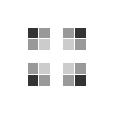
\begin{tikzpicture}[scale=0.3]
    \foreach \i in {0,...,4}
      \foreach \j in {0,...,4}
        \pgfmathparse{abs(\i-2)*abs(\j-2)*20}
        \fill[black!\pgfmathresult] (\i*0.5, -\j*0.5) rectangle ++(0.45, 0.45);
  \end{tikzpicture}
};

\node (vis2) at (7.0, 1.1) {
  
\begin{tikzpicture}[scale=0.3]
    \foreach \i in {0,...,4}
      \foreach \j in {0,...,4}
        \pgfmathparse{sin(deg(\i*1.5+\j*1.5))*50+50}
        \fill[black!\pgfmathresult] (\i*0.5, -\j*0.5) rectangle ++(0.45, 0.45);
  \end{tikzpicture}\quad
  
\begin{tikzpicture}[scale=0.3]
    \foreach \i in {0,...,4}
      \foreach \j in {0,...,4}
        \pgfmathparse{cos(deg(\i*2))*cos(deg(\j*2))*50+50}
        \fill[black!\pgfmathresult] (\i*0.5, -\j*0.5) rectangle ++(0.45, 0.45);
  \end{tikzpicture}\quad
  
\begin{tikzpicture}[scale=0.3]
    \foreach \i in {0,...,4}
      \foreach \j in {0,...,4}
        \pgfmathparse{sin(deg(sqrt(\i^2+\j^2)*2))*50+50}
        \fill[black!\pgfmathresult] (\i*0.5, -\j*0.5) rectangle ++(0.45, 0.45);
  \end{tikzpicture}
};

\node (vis3) at (10.5, 1.1) {
  
\begin{tikzpicture}[scale=0.3]
    \foreach \i in {0,...,4}
      \foreach \j in {0,...,4}
        \pgfmathparse{\i==2 && \j==2 ? 80 : 10}
        \fill[black!\pgfmathresult] (\i*0.5, -\j*0.5) rectangle ++(0.45, 0.45);
  \end{tikzpicture}\quad
  
\begin{tikzpicture}[scale=0.3]
    \foreach \i in {0,...,4}
      \foreach \j in {0,...,4}
        \pgfmathparse{(\i-2)^2+(\j-2)^2 < 2 ? 80 : 10}
        \fill[black!\pgfmathresult] (\i*0.5, -\j*0.5) rectangle ++(0.45, 0.45);
  \end{tikzpicture}\quad
  
\begin{tikzpicture}[scale=0.3]
    \foreach \i in {0,...,4}
      \foreach \j in {0,...,4}
        \pgfmathparse{(\i==1 || \i==3) && (\j>=1 && \j<=3) ? 80 : 10}
        \fill[black!\pgfmathresult] (\i*0.5, -\j*0.5) rectangle ++(0.45, 0.45);
  \end{tikzpicture}
};

% --- SETAS PONTILHADAS ---
\draw[->, draw=wp-muted, thick, dashed] (conv1.south) -- (vis1.north);
\draw[->, draw=wp-muted, thick, dashed] (conv2.south) -- (vis2.north);
\draw[->, draw=wp-muted, thick, dashed] (conv3.south) -- (vis3.north);


% --- TEXTOS INFERIORES DE CARACTERÍSTICAS ---
\node[font=\footnotesize, align=center, text=wp-accent] at (3.5, -0.1) {Bordas\\Texturas\\Cores};
\node[font=\footnotesize, align=center, text=wp-primary] at (7.0, -0.1) {Padrões\\Partes\\Formas simples};
\node[font=\footnotesize, align=center, text=wp-text] at (10.5, -0.1) {Objetos\\Semântica\\Conceitos};


% --- CHAVES SUPERIORES (Braces) ---
\draw[brk] (5.1, 4.0) -- (1.9, 4.0);
\node[above=4pt, font=\small, text=wp-accent] at (3.5, 4.0) {ESTILO (baixo nível)};

\draw[brk] (8.6, 4.0) -- (5.4, 4.0);
\node[above=4pt, font=\small, text=wp-primary] at (7.0, 4.0) {transição};

\draw[brk] (12.1, 4.0) -- (8.9, 4.0);
\node[above=4pt, font=\small, text=wp-text] at (10.5, 4.0) {CONTEÚDO (alto nível)};


% =========================================================================
% BLOCO SUPERIOR RE-ALINHADO E PROPORCIONAL
% Centrado exatamente em x=7.0 (meio do gráfico) com largura equilibrada de 7.0cm
% =========================================================================
\node[tuftebox, minimum width=7.0cm, minimum height=1.2cm] at (7.0, 6.0) {
    \textbf{\color{wp-primary}\small Extração de Características e Perdas}\\[4pt]
    \footnotesize Perda de estilo: múltiplas camadas (baixo + médio)\\
    \footnotesize Perda de conteúdo: camada profunda (alto nível)
};

\end{tikzpicture}
}
\caption{Hierarquia de características em uma CNN. Camadas iniciais capturam bordas, texturas e cores (estilo). Camadas médias detectam padrões e partes de objetos. Camadas profundas representam objetos completos e semântica de alto nível (conteúdo). A perda de estilo utiliza múltiplas camadas iniciais e médias, enquanto a perda de conteúdo utiliza uma camada profunda.}
\label{fig:cnn-hierarchy}
\end{figure}
\begin{figure}[htbp]
\centering
\resizebox{\textwidth}{!}{%
\begin{tikzpicture}[
    >=latex,
    layer/.style={draw=wp-text, rounded corners=2pt, minimum width=3.0cm, minimum height=1.2cm, align=center, font=\small},
    conn/.style={->, draw=wp-primary, thick},
    brk/.style={decorate, decoration={brace, amplitude=5pt}, draw=wp-muted, thick},
    tuftebox/.style={draw=wp-light, fill=wp-code, rounded corners=2pt, align=center}
]

% =========================================================================
% FLUXO PRINCIPAL: CAMADAS DA CNN (Eixo X Otimizado)
% =========================================================================

\node[layer, fill=wp-accent!15, draw=wp-accent] (conv1) at (3.5, 2.5) {Camadas Iniciais\\conv$_1$ -- conv$_2$};
\node[layer, fill=wp-primary!10, draw=wp-primary] (conv2) at (7.0, 2.5) {Camadas Médias\\conv$_3$ -- conv$_4$};
\node[layer, fill=wp-text!10, draw=wp-text] (conv3) at (10.5, 2.5) {Camadas Profundas\\conv$_5$ -- conv$_6$};

% Imagem de Entrada simplificada para apenas "X"
\node[draw=wp-text, fill=wp-code, rounded corners=2pt, minimum width=1.0cm, minimum height=1.0cm, align=center, font=\large\bfseries] (input) at (0.8, 2.5) {$\mathcal{I}$};

% Conexões do Fluxo Principal
\draw[->, draw=wp-primary, thick] (input.east) -- (conv1.west);
\draw[->, draw=wp-primary, thick] (conv1.east) -- (conv2.west);
\draw[->, draw=wp-primary, thick] (conv2.east) -- (conv3.west);


% =========================================================================
% VISUALIZAÇÕES DE RECURSOS (Aproximadas verticalmente)
% =========================================================================

\node (vis1) at (3.5, 1.1) {
  \begin{tikzpicture}[scale=0.3]
    \foreach \i in {0,...,4}
      \foreach \j in {0,...,4}
        \pgfmathparse{mod(\i+\j,2)*100}
        \fill[black!\pgfmathresult] (\i*0.5, -\j*0.5) rectangle ++(0.45, 0.45);
  \end{tikzpicture}\quad
  
\begin{tikzpicture}[scale=0.3]
    \foreach \i in {0,...,4}
      \foreach \j in {0,...,4}
        \pgfmathparse{int(rnd*100)}
        \fill[black!\pgfmathresult] (\i*0.5, -\j*0.5) rectangle ++(0.45, 0.45);
  \end{tikzpicture}\quad
  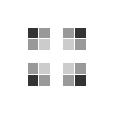
\begin{tikzpicture}[scale=0.3]
    \foreach \i in {0,...,4}
      \foreach \j in {0,...,4}
        \pgfmathparse{abs(\i-2)*abs(\j-2)*20}
        \fill[black!\pgfmathresult] (\i*0.5, -\j*0.5) rectangle ++(0.45, 0.45);
  \end{tikzpicture}
};

\node (vis2) at (7.0, 1.1) {
  
\begin{tikzpicture}[scale=0.3]
    \foreach \i in {0,...,4}
      \foreach \j in {0,...,4}
        \pgfmathparse{sin(deg(\i*1.5+\j*1.5))*50+50}
        \fill[black!\pgfmathresult] (\i*0.5, -\j*0.5) rectangle ++(0.45, 0.45);
  \end{tikzpicture}\quad
  
\begin{tikzpicture}[scale=0.3]
    \foreach \i in {0,...,4}
      \foreach \j in {0,...,4}
        \pgfmathparse{cos(deg(\i*2))*cos(deg(\j*2))*50+50}
        \fill[black!\pgfmathresult] (\i*0.5, -\j*0.5) rectangle ++(0.45, 0.45);
  \end{tikzpicture}\quad
  
\begin{tikzpicture}[scale=0.3]
    \foreach \i in {0,...,4}
      \foreach \j in {0,...,4}
        \pgfmathparse{sin(deg(sqrt(\i^2+\j^2)*2))*50+50}
        \fill[black!\pgfmathresult] (\i*0.5, -\j*0.5) rectangle ++(0.45, 0.45);
  \end{tikzpicture}
};

\node (vis3) at (10.5, 1.1) {
  
\begin{tikzpicture}[scale=0.3]
    \foreach \i in {0,...,4}
      \foreach \j in {0,...,4}
        \pgfmathparse{\i==2 && \j==2 ? 80 : 10}
        \fill[black!\pgfmathresult] (\i*0.5, -\j*0.5) rectangle ++(0.45, 0.45);
  \end{tikzpicture}\quad
  
\begin{tikzpicture}[scale=0.3]
    \foreach \i in {0,...,4}
      \foreach \j in {0,...,4}
        \pgfmathparse{(\i-2)^2+(\j-2)^2 < 2 ? 80 : 10}
        \fill[black!\pgfmathresult] (\i*0.5, -\j*0.5) rectangle ++(0.45, 0.45);
  \end{tikzpicture}\quad
  
\begin{tikzpicture}[scale=0.3]
    \foreach \i in {0,...,4}
      \foreach \j in {0,...,4}
        \pgfmathparse{(\i==1 || \i==3) && (\j>=1 && \j<=3) ? 80 : 10}
        \fill[black!\pgfmathresult] (\i*0.5, -\j*0.5) rectangle ++(0.45, 0.45);
  \end{tikzpicture}
};

% --- SETAS PONTILHADAS ---
\draw[->, draw=wp-muted, thick, dashed] (conv1.south) -- (vis1.north);
\draw[->, draw=wp-muted, thick, dashed] (conv2.south) -- (vis2.north);
\draw[->, draw=wp-muted, thick, dashed] (conv3.south) -- (vis3.north);


% --- TEXTOS INFERIORES DE CARACTERÍSTICAS ---
\node[font=\footnotesize, align=center, text=wp-accent] at (3.5, -0.1) {Bordas\\Texturas\\Cores};
\node[font=\footnotesize, align=center, text=wp-primary] at (7.0, -0.1) {Padrões\\Partes\\Formas simples};
\node[font=\footnotesize, align=center, text=wp-text] at (10.5, -0.1) {Objetos\\Semântica\\Conceitos};


% --- CHAVES SUPERIORES (Braces) ---
\draw[brk] (5.1, 4.0) -- (1.9, 4.0);
\node[above=4pt, font=\small, text=wp-accent] at (3.5, 4.0) {ESTILO (baixo nível)};

\draw[brk] (8.6, 4.0) -- (5.4, 4.0);
\node[above=4pt, font=\small, text=wp-primary] at (7.0, 4.0) {transição};

\draw[brk] (12.1, 4.0) -- (8.9, 4.0);
\node[above=4pt, font=\small, text=wp-text] at (10.5, 4.0) {CONTEÚDO (alto nível)};


% =========================================================================
% BLOCO SUPERIOR RE-ALINHADO E PROPORCIONAL
% Centrado exatamente em x=7.0 (meio do gráfico) com largura equilibrada de 7.0cm
% =========================================================================
\node[tuftebox, minimum width=7.0cm, minimum height=1.2cm] at (7.0, 6.0) {
    \textbf{\color{wp-primary}\small Extração de Características e Perdas}\\[4pt]
    \footnotesize Perda de estilo: múltiplas camadas (baixo + médio)\\
    \footnotesize Perda de conteúdo: camada profunda (alto nível)
};

\end{tikzpicture}
}
\caption{Hierarquia de características em uma CNN. Camadas iniciais capturam bordas, texturas e cores (estilo). Camadas médias detectam padrões e partes de objetos. Camadas profundas representam objetos completos e semântica de alto nível (conteúdo). A perda de estilo utiliza múltiplas camadas iniciais e médias, enquanto a perda de conteúdo utiliza uma camada profunda.}
\label{fig:cnn-hierarchy}
\end{figure}
\begin{figure}[htbp]
\centering
\resizebox{\textwidth}{!}{%
\begin{tikzpicture}[
    >=latex,
    layer/.style={draw=wp-text, rounded corners=2pt, minimum width=3.0cm, minimum height=1.2cm, align=center, font=\small},
    conn/.style={->, draw=wp-primary, thick},
    brk/.style={decorate, decoration={brace, amplitude=5pt}, draw=wp-muted, thick},
    tuftebox/.style={draw=wp-light, fill=wp-code, rounded corners=2pt, align=center}
]

% =========================================================================
% FLUXO PRINCIPAL: CAMADAS DA CNN (Eixo X Otimizado)
% =========================================================================

\node[layer, fill=wp-accent!15, draw=wp-accent] (conv1) at (3.5, 2.5) {Camadas Iniciais\\conv$_1$ -- conv$_2$};
\node[layer, fill=wp-primary!10, draw=wp-primary] (conv2) at (7.0, 2.5) {Camadas Médias\\conv$_3$ -- conv$_4$};
\node[layer, fill=wp-text!10, draw=wp-text] (conv3) at (10.5, 2.5) {Camadas Profundas\\conv$_5$ -- conv$_6$};

% Imagem de Entrada simplificada para apenas "X"
\node[draw=wp-text, fill=wp-code, rounded corners=2pt, minimum width=1.0cm, minimum height=1.0cm, align=center, font=\large\bfseries] (input) at (0.8, 2.5) {$\mathcal{I}$};

% Conexões do Fluxo Principal
\draw[->, draw=wp-primary, thick] (input.east) -- (conv1.west);
\draw[->, draw=wp-primary, thick] (conv1.east) -- (conv2.west);
\draw[->, draw=wp-primary, thick] (conv2.east) -- (conv3.west);


% =========================================================================
% VISUALIZAÇÕES DE RECURSOS (Aproximadas verticalmente)
% =========================================================================

\node (vis1) at (3.5, 1.1) {
  \begin{tikzpicture}[scale=0.3]
    \foreach \i in {0,...,4}
      \foreach \j in {0,...,4}
        \pgfmathparse{mod(\i+\j,2)*100}
        \fill[black!\pgfmathresult] (\i*0.5, -\j*0.5) rectangle ++(0.45, 0.45);
  \end{tikzpicture}\quad
  
\begin{tikzpicture}[scale=0.3]
    \foreach \i in {0,...,4}
      \foreach \j in {0,...,4}
        \pgfmathparse{int(rnd*100)}
        \fill[black!\pgfmathresult] (\i*0.5, -\j*0.5) rectangle ++(0.45, 0.45);
  \end{tikzpicture}\quad
  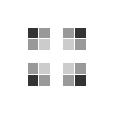
\begin{tikzpicture}[scale=0.3]
    \foreach \i in {0,...,4}
      \foreach \j in {0,...,4}
        \pgfmathparse{abs(\i-2)*abs(\j-2)*20}
        \fill[black!\pgfmathresult] (\i*0.5, -\j*0.5) rectangle ++(0.45, 0.45);
  \end{tikzpicture}
};

\node (vis2) at (7.0, 1.1) {
  
\begin{tikzpicture}[scale=0.3]
    \foreach \i in {0,...,4}
      \foreach \j in {0,...,4}
        \pgfmathparse{sin(deg(\i*1.5+\j*1.5))*50+50}
        \fill[black!\pgfmathresult] (\i*0.5, -\j*0.5) rectangle ++(0.45, 0.45);
  \end{tikzpicture}\quad
  
\begin{tikzpicture}[scale=0.3]
    \foreach \i in {0,...,4}
      \foreach \j in {0,...,4}
        \pgfmathparse{cos(deg(\i*2))*cos(deg(\j*2))*50+50}
        \fill[black!\pgfmathresult] (\i*0.5, -\j*0.5) rectangle ++(0.45, 0.45);
  \end{tikzpicture}\quad
  
\begin{tikzpicture}[scale=0.3]
    \foreach \i in {0,...,4}
      \foreach \j in {0,...,4}
        \pgfmathparse{sin(deg(sqrt(\i^2+\j^2)*2))*50+50}
        \fill[black!\pgfmathresult] (\i*0.5, -\j*0.5) rectangle ++(0.45, 0.45);
  \end{tikzpicture}
};

\node (vis3) at (10.5, 1.1) {
  
\begin{tikzpicture}[scale=0.3]
    \foreach \i in {0,...,4}
      \foreach \j in {0,...,4}
        \pgfmathparse{\i==2 && \j==2 ? 80 : 10}
        \fill[black!\pgfmathresult] (\i*0.5, -\j*0.5) rectangle ++(0.45, 0.45);
  \end{tikzpicture}\quad
  
\begin{tikzpicture}[scale=0.3]
    \foreach \i in {0,...,4}
      \foreach \j in {0,...,4}
        \pgfmathparse{(\i-2)^2+(\j-2)^2 < 2 ? 80 : 10}
        \fill[black!\pgfmathresult] (\i*0.5, -\j*0.5) rectangle ++(0.45, 0.45);
  \end{tikzpicture}\quad
  
\begin{tikzpicture}[scale=0.3]
    \foreach \i in {0,...,4}
      \foreach \j in {0,...,4}
        \pgfmathparse{(\i==1 || \i==3) && (\j>=1 && \j<=3) ? 80 : 10}
        \fill[black!\pgfmathresult] (\i*0.5, -\j*0.5) rectangle ++(0.45, 0.45);
  \end{tikzpicture}
};

% --- SETAS PONTILHADAS ---
\draw[->, draw=wp-muted, thick, dashed] (conv1.south) -- (vis1.north);
\draw[->, draw=wp-muted, thick, dashed] (conv2.south) -- (vis2.north);
\draw[->, draw=wp-muted, thick, dashed] (conv3.south) -- (vis3.north);


% --- TEXTOS INFERIORES DE CARACTERÍSTICAS ---
\node[font=\footnotesize, align=center, text=wp-accent] at (3.5, -0.1) {Bordas\\Texturas\\Cores};
\node[font=\footnotesize, align=center, text=wp-primary] at (7.0, -0.1) {Padrões\\Partes\\Formas simples};
\node[font=\footnotesize, align=center, text=wp-text] at (10.5, -0.1) {Objetos\\Semântica\\Conceitos};


% --- CHAVES SUPERIORES (Braces) ---
\draw[brk] (5.1, 4.0) -- (1.9, 4.0);
\node[above=4pt, font=\small, text=wp-accent] at (3.5, 4.0) {ESTILO (baixo nível)};

\draw[brk] (8.6, 4.0) -- (5.4, 4.0);
\node[above=4pt, font=\small, text=wp-primary] at (7.0, 4.0) {transição};

\draw[brk] (12.1, 4.0) -- (8.9, 4.0);
\node[above=4pt, font=\small, text=wp-text] at (10.5, 4.0) {CONTEÚDO (alto nível)};


% =========================================================================
% BLOCO SUPERIOR RE-ALINHADO E PROPORCIONAL
% Centrado exatamente em x=7.0 (meio do gráfico) com largura equilibrada de 7.0cm
% =========================================================================
\node[tuftebox, minimum width=7.0cm, minimum height=1.2cm] at (7.0, 6.0) {
    \textbf{\color{wp-primary}\small Extração de Características e Perdas}\\[4pt]
    \footnotesize Perda de estilo: múltiplas camadas (baixo + médio)\\
    \footnotesize Perda de conteúdo: camada profunda (alto nível)
};

\end{tikzpicture}
}
\caption{Hierarquia de características em uma CNN. Camadas iniciais capturam bordas, texturas e cores (estilo). Camadas médias detectam padrões e partes de objetos. Camadas profundas representam objetos completos e semântica de alto nível (conteúdo). A perda de estilo utiliza múltiplas camadas iniciais e médias, enquanto a perda de conteúdo utiliza uma camada profunda.}
\label{fig:cnn-hierarchy}
\end{figure}